\documentclass[10pt]{article}

\usepackage{amsthm}
\usepackage{amsmath}
\usepackage{amssymb}
\usepackage{mathtools}
\usepackage{graphicx}
\usepackage[colorinlistoftodos]{todonotes}
\usepackage{url}
\usepackage{xcolor}
\usepackage[font=small,labelfont=bf]{caption}

\usepackage{pgfplots}

\usepackage[left = 1cm, top = 1cm, bottom = 2cm, right = 1cm, nohead, nofoot]{geometry}

\pgfplotsset{width=20cm, compat=1.9}

\newcommand{\C}{\mathbb{C}}  % Complex
\newcommand{\R}{\mathbb{R}}  % Real
\newcommand{\Z}{\mathbb{Z}}  % Integers
\newcommand{\N}{\mathbb{N}}  % Naturals

\newcommand{\A}{\mathbb{A}}
\newcommand{\K}{\mathbb{K}}

\title{$\A$dvanced $\C$alculus}
\author{$\C$ason $\K$onzer}
\date{November 13, 2021}



\begin{document}
\maketitle

\newpage

%%%%%%%%%%%%%%%%%%%%%%%%%%%%%%%%%%%%%%%%%%%%%%%%%%%%%%%%%%%%%%%%%%%%%%%%%%%%%%%%%%%%%%%%%%%%%%%%
%%%%%%%%%%%%%%%%%%%%%%%%%%%%%%%%%%        Problem #1       %%%%%%%%%%%%%%%%%%%%%%%%%%%%%%%%%%%%%
\section{\underline{}}
\label{sec: Problem 1}

\noindent
Find the Fourier series representation of $ u(x,t) $, the solution to the wave equation with 
$ c = 1 $, $ L = 1 $, $ g(x) = 0 $, and $ f(x) = 0.01x(1 - x) $ on $ 0 \le x < 1 $, extended as an odd function. 
List the first 4 non-zero terms. You may use Mathematica to find $ B_n $ but only if you submit the notebook file showing your work. \\
\vspace{2.5mm}

\hrule 

\vspace{7.5mm}

\begin{itemize}
    \item \textit{Solution via seperation of variables:} $ \displaystyle u(x,t) = \sum_{n = 1}^{\infty} u_n(x,t) $
    \subitem $ \displaystyle u_n(x,t) = (B_{n}\cos{\lambda_{n}t} + B^{*}_{n}\sin{\lambda_{n}t})\sin{\dfrac{n\pi x}{L}} $
    \subitem $ \displaystyle B_{n} =  \dfrac{2}{L} \int_{0}^{L} f(x)\sin{\dfrac{n\pi x}{L}} \,dx $
    \subitem $ \displaystyle B^{*}_{n} = \dfrac{2}{cn\pi} \int_{0}^{L} g(x)\sin{\dfrac{n\pi x}{L}} \,dx $
    \subitem $ \displaystyle \lambda_{n} = \dfrac{cn\pi}{L} $
    \item Solving for given values.. Integration in corresponding notebook
    \subitem $ \displaystyle \lambda_{n} = \dfrac{1n\pi}{1} = n\pi $
    \subitem $ \displaystyle B^{*}_{n} = \dfrac{2}{1n\pi} \int_{0}^{1} 0\sin{\dfrac{1\pi x}{1}} \,dx = 0 $
    \subitem $ \displaystyle B_{n} = \dfrac{2}{1} \int_{0}^{1} (0.01x - 0.01x^{2})\sin{\dfrac{n\pi x}{1}} \,dx = 0.02 \Bigl[ \int_{0}^{1} x\sin{n\pi x} \,dx - \int_{0}^{1} x^{2}\sin{n\pi x} \,dx \Bigr] $
    \subitem $ \displaystyle B_{n} = 0.02\Bigl[\dfrac{(\pi  n) \sin -\pi  n ((\pi  n) \cos )}{\pi ^2 n^2}-\dfrac{\left(2-\pi ^2 n^2\right) ((\pi  n) \cos )+2 \pi  n ((\pi  n) \sin )-2}{\pi ^3 n^3}\Bigr] $
    \subitem $ \displaystyle u_n(x,t) = \Bigl(0.02\Bigl[\dfrac{(\pi  n) \sin -\pi  n ((\pi  n) \cos )}{\pi ^2 n^2}-\dfrac{\left(2-\pi ^2 n^2\right) ((\pi  n) \cos )+2 \pi  n ((\pi  n) \sin )-2}{\pi ^3 n^3}\Bigr]\cos{n\pi t} + 0\sin{n\pi t}\Bigr)\sin{\dfrac{n\pi x}{1}} $
    \subitem $ \displaystyle u_n(x,t) = 0.02\Bigl(\Bigl[\dfrac{(\pi  n) \sin -\pi  n ((\pi  n) \cos )}{\pi ^2 n^2}-\dfrac{\left(2-\pi ^2 n^2\right) ((\pi  n) \cos )+2 \pi  n ((\pi  n) \sin )-2}{\pi ^3 n^3}\Bigr]\cos{n\pi t}\Bigr)\sin{n\pi x} $
    \subitem $ \displaystyle u(x,t) = 0.02 \sum_{n = 1}^{\infty} \Bigl(\Bigl[\dfrac{(\pi  n) \sin -\pi  n ((\pi  n) \cos )}{\pi ^2 n^2}-\dfrac{\left(2-\pi ^2 n^2\right) ((\pi  n) \cos )+2 \pi  n ((\pi  n) \sin )-2}{\pi ^3 n^3}\Bigr]\cos{n\pi t}\Bigr)\sin{n\pi x} $
    \item Solving for first 4 non-zero terms.. Table in corresponding notebook
    \subitem $ n = 1 \ : \ 0.00258012\cos{\pi t}\sin{\pi x} $
    \subitem $ n = 3 \ : \ 0.0000955601\cos{3\pi t}\sin{3\pi x} $
    \subitem $ n = 5 \ : \ 0.000020641\cos{5\pi t}\sin{5\pi x} $
    \subitem $ n = 7 \ : \ 7.52222*10^{-6}\cos{7\pi t}\sin{7\pi x} $
    \item Approximate solution up to n = 8
    \subitem  $ \displaystyle u_n(x,t) = 0.00258\cos{\pi t}\sin{\pi x} + 0.0000956\cos{3\pi t}\sin{3\pi x} + 0.000021\cos{5\pi t}\sin{5\pi x} + 7.52*10^{-6}\cos{7\pi t}\sin{7\pi x} $
\end{itemize}

\newpage

%%%%%%%%%%%%%%%%%%%%%%%%%%%%%%%%%%%%%%%%%%%%%%%%%%%%%%%%%%%%%%%%%%%%%%%%%%%%%%%%%%%%%%%%%%%%%%%%
%%%%%%%%%%%%%%%%%%%%%%%%%%%%%%%%%%        Problem #2       %%%%%%%%%%%%%%%%%%%%%%%%%%%%%%%%%%%%%
\section{\underline{}}
\label{sec: Problem 2}

\noindent
Using your solution to \#1, plot $ f(x) $, $ u(x,0) $, and $ u(x,0.5) $ on the same graph.  \\
\vspace{2.5mm}

\hrule 

\vspace{7.5mm}
\begin{center}
    \begin{minipage}{0.75\linewidth}
        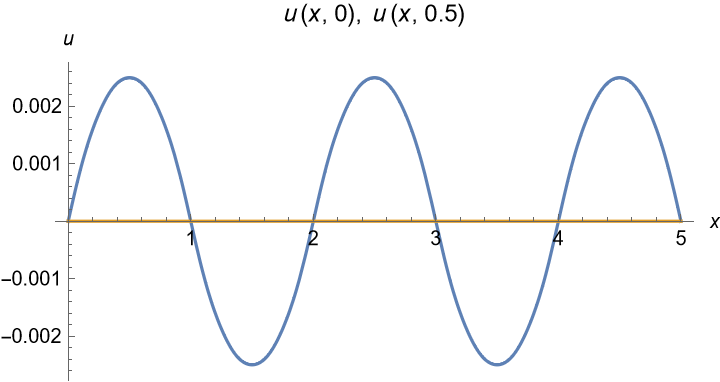
\includegraphics[width=\textwidth]{IMG/2.png}
        \captionof{figure}{static time}
    \end{minipage} \\
    \vspace{5mm}
    \begin{minipage}{0.75\linewidth}
        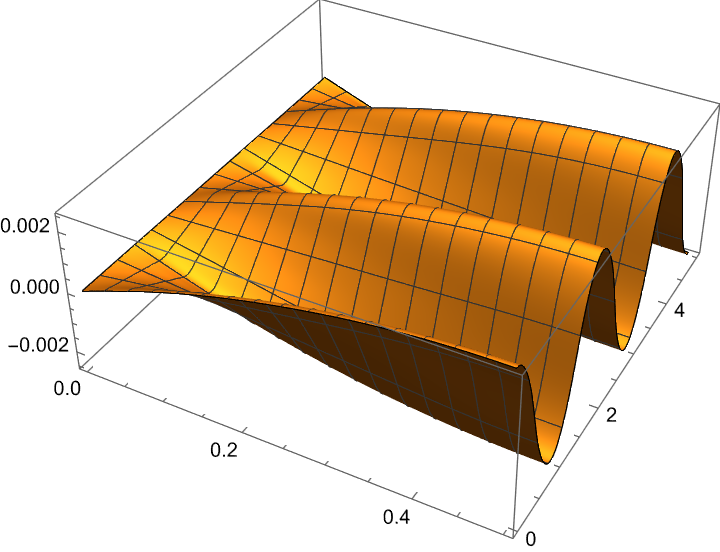
\includegraphics[width=\textwidth]{IMG/2-.png}
        \captionof{figure}{dynamic time}
    \end{minipage}
\end{center}
\newpage

%%%%%%%%%%%%%%%%%%%%%%%%%%%%%%%%%%%%%%%%%%%%%%%%%%%%%%%%%%%%%%%%%%%%%%%%%%%%%%%%%%%%%%%%%%%%%%%%
%%%%%%%%%%%%%%%%%%%%%%%%%%%%%%%%%%        Problem #3       %%%%%%%%%%%%%%%%%%%%%%%%%%%%%%%%%%%%%
\section{\underline{}}
\label{sec: Problem 3}

\noindent
Using D'Alembert's solution to \#1 (i.e. $ u(x,t) = \frac{1}{2}(f(x + t) + f(x - t)) $), plot $ u(x,t) $, $ \frac{1}{2}f(x + t) $, 
and $ \frac{1}{2}f(x - t) $ on the same graph, creating one graph  for each of $ t = 0, 0.2., 0.4, 0.6, 0.8, $ and $ 1. $ 
You probably want to use Mathematica for this. Note, you MUST extend $f (x) $ to be odd with period 2. \\
\vspace{2.5mm}

\hrule 

\vspace{7.5mm}

\begin{center}
    \begin{minipage}{0.48\linewidth}
        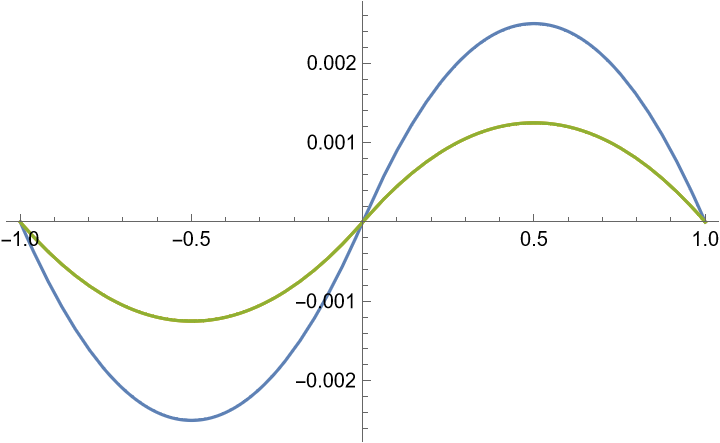
\includegraphics[width=\textwidth]{IMG/3-0.0.png}
        \captionof{figure}{t=0.0}
    \end{minipage}
    \hfill
    \begin{minipage}{0.49\linewidth}
        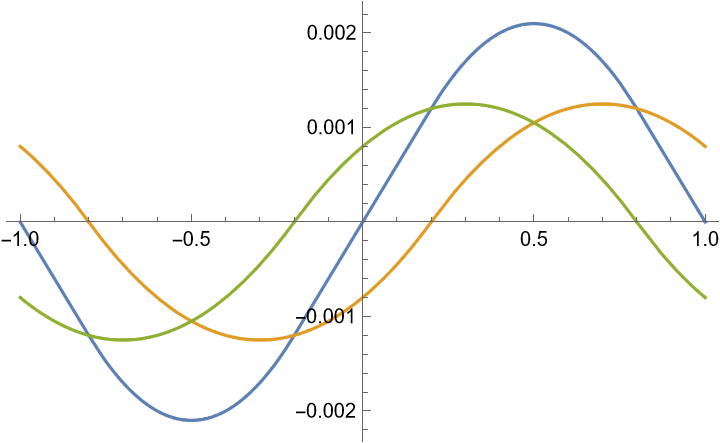
\includegraphics[width=\textwidth]{IMG/3-0.2.png}
        \captionof{figure}{t=0.2}
    \end{minipage}
\end{center}
\begin{center}
    \begin{minipage}{0.49\linewidth}
        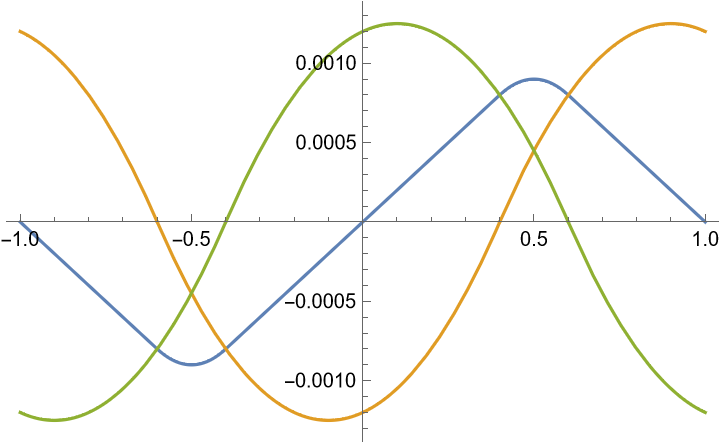
\includegraphics[width=\textwidth]{IMG/3-0.4.png}
        \captionof{figure}{t=0.4}
    \end{minipage}
    \hfill
    \begin{minipage}{0.49\linewidth}
        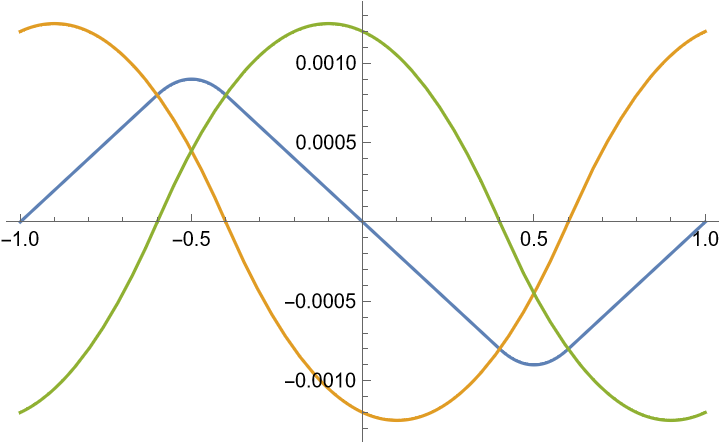
\includegraphics[width=\textwidth]{IMG/3-0.6.png}
        \captionof{figure}{t=0.6}
    \end{minipage}
\end{center}
\begin{center}
    \begin{minipage}{0.49\linewidth}
        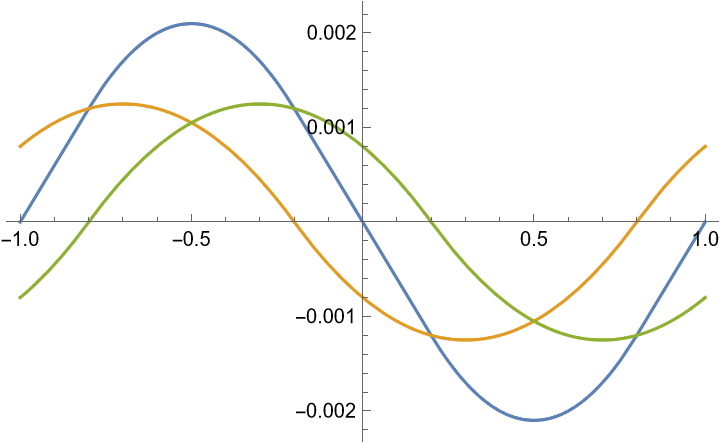
\includegraphics[width=\textwidth]{IMG/3-0.8.png}
        \captionof{figure}{t=0.8}
    \end{minipage}
    \hfill
    \begin{minipage}{0.49\linewidth}
        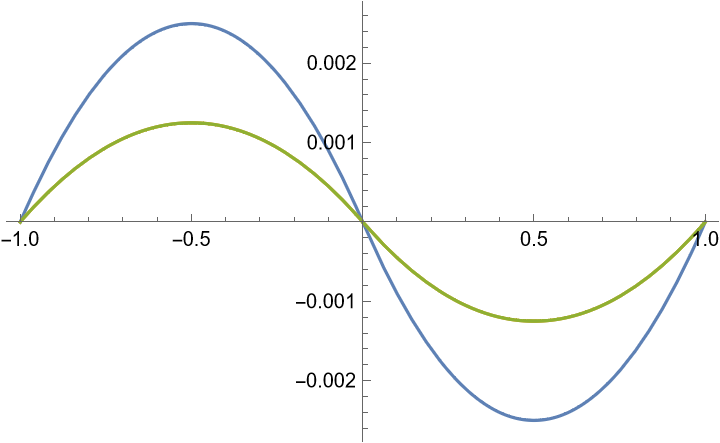
\includegraphics[width=\textwidth]{IMG/3-1.0.png}
        \captionof{figure}{t=1.0}
    \end{minipage}
\end{center}

\newpage

\end{document}


%%%%%%%%%%%%%%%%%%%%%%%%%%%%%%%%%%%%%%%%%%%%%%%%%%%%%%%%%%%%%%%%%%%%%%%%%%%%%%%%%%%%%%%%%%%%%%%%
%%%%%%%%%%%%%  Comments - November 13, 2021 Advanced Calculus Written Home Work #7  %%%%%%%%%%%%%